\section{曲面上的直线}\label{sec:lines-on-surfaces}

在本书最后两节中, 我们研究曲面上的直线, 最终目的是证明一个经典事实: 每个光滑三次曲面恰好包含 $27$ 条直线. 实际上, 证明这个经典结果时最棘手的部分之一, 是证明每个三次曲面至少包含一条直线; 本节将把这一事实作为纤维维数定理的应用来证明. 为此, 先退一步, 明确我们所说的 $\mathbb{P}^{3}$ 中曲面的次数是什么意思.

就接下来的两节而言, $\mathbb{P}^{3}$ 中的曲面指任意二维不可约射影簇 $X\subseteq\mathbb{P}^{3}$. 若 $X\subseteq\mathbb{P}^{3}$ 是一个曲面, 则 $\mathcal{I}(X)$ 是由任意在 $X$ 上消没的不可约多项式生成的主理想 (Exercise~\ref{ex:vanishing-ideal-of-pure-codimension-one-projective-variety-is-principal}). 由于主理想的任意两个生成元只相差一个标量因子, 以下概念是良定义的.

\begin{Definition}{$\mathbb{P}^{3}$ 中曲面的次数}\leavevmode\label{def:degree-of-surface-in-projective-three-space}
令 $X\subseteq\mathbb{P}^{3}$ 为一个曲面. $X$ 在 $\mathbb{P}^{3}$ 中的\emph{次数}是 $\mathcal{I}(X)$ 任一生成元的多项式次数.
\end{Definition}

\BookPairedNote{
更一般地, 可以定义任意射影簇 $X\subseteq\mathbb{P}^{n}$ 的次数. 对 $\mathbb{P}^{n}$ 中的超曲面 $X$, 次数就是 $\mathcal{I}(X)$ 任一生成元的次数. 但对于 $\mathbb{P}^{n}$ 中余维更高的射影簇, 次数的概念要复杂一些, 不那么容易精确定义.
}{
直观上, $\mathbb{P}^{n}$ 中一个簇的次数衡量的是它有多\textquotedbl{}弯曲\textquotedbl{}.
}

由于生成曲面 $X\subseteq\mathbb{P}^{3}$ 的消没理想的两个多项式只相差一个标量因子, 我们现在换一个角度, 不再考虑曲面, 而直接研究在相差非零标量因子的意义下的多项式.

\begin{BookNotation}[$\ensuremath{K[x_{0},x_{1},x_{2},x_{3}]_{d}}$ 和 $\mathbb{P}_{3,d}$]\leavevmode\label{notation:projective-space-of-degree-d-polynomials}
令 $K[x_{0},x_{1},x_{2},x_{3}]_{d}$ 为 $K[x_{0},x_{1},x_{2},x_{3}]$ 中由 $d$ 次齐次多项式构成的线性子空间, 并定义
\[
  \mathbb{P}_{3,d}=\frac{K[x_{0},x_{1},x_{2},x_{3}]_{d}\setminus\{0\}}{\sim},
\]
其中当对某个 $\lambda\in K\setminus\{0\}$ 有 $f=\lambda g$ 时, $f\sim g$.
\end{BookNotation}

我们自然地将 $\mathbb{P}_{3,d}$ 等同于以 $K[x_{0},x_{1},x_{2},x_{3}]_{d}$ 中多项式的系数为坐标的射影空间:
\[
  \mathbb{P}_{3,d}=\mathbb{P}^{\binom{d+3}{3}-1}.
\]
每个 $d$ 次曲面自然对应射影空间 $\mathbb{P}_{3,d}$ 中的一个点: 若 $\mathcal{I}(X)=\langle f\rangle$, 就将 $X$ 与 $[f]\in\mathbb{P}_{3,d}$ 等同. 由前面的讨论可知, 这是良定义的. 然而, 并非 $\mathbb{P}_{3,d}$ 的每一点都对应 $\mathbb{P}^{3}$ 中的一个 $d$ 次曲面, 因为其中一些点, 例如 $[x_{0}^{d}]$, 对应可约多项式, 所以它们不定义 (不可约) 曲面.

虽说从研究 $d$ 次曲面的角度看, $\mathbb{P}_{3,d}$ 含有多余的点, 但加上这些点的好处是可以在一个射影空间中工作, 而不是在射影空间的一个子集中工作. 关于 $\mathbb{P}_{3,d}$ 中各点的统一结论, 一经证明, 应用到曲面所对应的点上, 就给出关于所有 $d$ 次曲面的结论.

作为研究曲面上直线的准备, 提醒读者, $\mathbb{P}^{3}$ 中的直线 $L$ 有几种不同的看法, 我们会交替使用:
\begin{itemize}
  \item 将它视为消没集 $\mathcal{V}(\ell_{0},\ell_{1})\subseteq\mathbb{P}^{3}$, 其中 $\ell_{0},\ell_{1}\in K[x_{0},x_{1},x_{2},x_{3}]_{1}$ 是一对线性无关的齐次线性多项式;
  \item 将它视为 $\mathbb{P}(V)=\dfrac{V\setminus\{0\}}{\sim}$, 其中 $V\subseteq K^{4}$ 是二维线性子空间;
  \item 将它视为单射的线性映射 $\mathbb{P}^{1}\to\mathbb{P}^{3}$ 的像.
\end{itemize}
还要回顾, $\mathbb{P}^{3}$ 中的直线由 Grassmann 簇 $\mathrm{G}(2,4)$ 参数化. 借助 Plücker 映射 (Section~\ref{sec:grassmannians-and-plucker-maps}), 我们把它看作 $\mathbb{P}^{5}$ 中的一个射影超曲面.

现在转向本节的主要问题: 给定 $[f]\in\mathbb{P}_{3,d}$, 曲面 $\mathcal{V}(f)\subseteq\mathbb{P}^{3}$ 是否包含一条直线? 先从 $d=3$ 的一个具体例子开始.

\begin{Example}{Fermat 三次曲面上的一条直线}\leavevmode\label{ex:line-on-fermat-cubic-surface}
\BookPairedFigure{
令 $K=\mathbb{C}$, 考察不可约三次多项式 $f=x_{0}^{3}+x_{1}^{3}+x_{2}^{3}+x_{3}^{3}$, 通常称为\textquotedbl{}Fermat 三次式\textquotedbl{}. 令 $L\subseteq\mathbb{P}^{3}$ 为由下式定义的直线:
\[
  L=\{[a:b:-a:-b]\mid [a:b]\in\mathbb{P}^{1}\}\subseteq\mathbb{P}^{3}.
\]
易验证 $f$ 在 $L$ 的每一点处消没, 因此 $L\subseteq\mathcal{V}(f)$.
}{
\phantomsection\label{fig:fermat-cubic-with-line}%
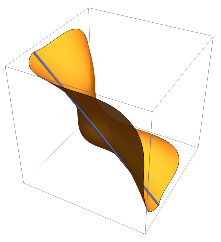
\includegraphics[width=\linewidth]{figures/fermat-cubic-with-line.pdf}
}
图中画出了 $\mathcal{V}(f)$ 和 $L$ 的仿射限制 (的实点).
\end{Example}

上一例给出了一个包含直线的特定三次曲面, 而我们的目标是证明每个三次曲面都包含一条直线. 后一个断言要难证得多. 为这一更一般的结论做准备, 先讨论比较初等的情形: 平面中的直线 ($d=1$) 和二次曲面中的直线 ($d=2$).

在 $d=1$ 时, 多项式 $f\in K[x_{0},x_{1},x_{2},x_{3}]_{1}$ 定义平面 $P=\mathcal{V}(f)\subseteq\mathbb{P}^{3}$. 由于每个平面都包含直线, 实际上, 每个平面都包含无穷多条由 $\mathrm{G}(2,3)\cong\mathbb{P}^{2}$ 参数化的直线, 所以对任意 $[f]\in\mathbb{P}_{3,1}$, 射影簇 $\mathcal{V}(f)\subseteq\mathbb{P}^{3}$ 包含无穷多条直线, 这些直线可由 $\mathbb{P}^{2}$ 参数化.

$d=2$ 的情形稍难一些, 我们在下一个结果中处理它.

\begin{Proposition}{二次曲面由直线覆盖}\leavevmode\label{prop:quadric-surfaces-are-covered-by-lines}
给定 $[f]\in\mathbb{P}_{3,2}$ 和 $a\in\mathcal{V}(f)$, 至少存在一条直线 $L\subseteq\mathbb{P}^{3}$, 使 $a\in L\subseteq\mathcal{V}(f)$. 特别地, $\mathcal{V}(f)$ 包含无穷多条直线.
\end{Proposition}
\begin{Proof}
令 $f\in K[x_{0},x_{1},x_{2},x_{3}]_{2}$ 为齐次二次多项式, 令 $a\in\mathcal{V}(f)\subseteq\mathbb{P}^{3}$. 写 $a=[a_{0}:a_{1}:a_{2}:a_{3}]$, 不妨设 $a_{0}=1$. 限制在仿射开片 $\mathbb{A}_{0}^{3}=\mathbb{A}^{3}$ 上, $\mathbb{P}^{3}$ 中经过 $a$ 的任意直线都由其仿射限制唯一确定, 此仿射限制是形如
\[
  L_{b}=\{(a_{1},a_{2},a_{3})+t(b_{1},b_{2},b_{3})\mid t\in K\}
\]
的仿射直线, 其中 $b=(b_{1},b_{2},b_{3})\ne(0,0,0)$. 由于 $L_{b}$ 不随 $b$ 的缩放而改变, 我们将 $b=[b_{1}:b_{2}:b_{3}]$ 视为 $\mathbb{P}^{2}$ 的元素.

若 $L$ 是经过 $a$ 的一条直线, 则 $f$ 在 $L$ 上消没当且仅当 $f_{0}=f(1,x_{1},x_{2},x_{3})$ 在 $L$ 的仿射限制上消没. 在这样的仿射限制 $L_{b}$ 的每一点上对 $f_{0}$ 求值, 并合并 $t$ 的同次幂, 得到形如
\begin{equation}\label{eq:degree-two-restriction-to-affine-line-through-point}
  f_{0}(a_{1}+tb_{1},a_{2}+tb_{2},a_{3}+tb_{3})
  =g_{1}(b_{1},b_{2},b_{3})t+g_{2}(b_{1},b_{2},b_{3})t^{2},
\end{equation}
的式子, 其中 $g_{i}$ 是 $i$ 次齐次的, 而 $t^{0}$ 项为零, 因为 $f_{0}(a_{1},a_{2},a_{3})=0$. 因此, $f_{0}$ 在 $L_{b}$ 上消没当且仅当 $b\in\mathcal{V}(g_{1},g_{2})$. 由于任意两个齐次多项式在 $\mathbb{P}^{2}$ 中的公共消没集非空 (Proposition~\ref{prop:dimension-of-homogeneous-systems}), 至少存在一个解 $b\in\mathcal{V}(g_{1},g_{2})\in\mathbb{P}^{2}$, 从而至少存在一条直线 $L=\overline{L_{b}}\subseteq\mathbb{P}^{3}$, 使 $a\in L\subseteq\mathcal{V}(f)$.

于是可得命题的最后一个断言: 若 $\mathcal{V}(f)$ 上只有有限多条直线, 由于 $\mathcal{V}(f)$ 的每一点都在其中一条直线上, $\mathcal{V}(f)$ 就会是有限多条直线的并, 与它是二维的矛盾.
\end{Proof}

\begin{Example}{二次曲面上的直线}\leavevmode\label{ex:lines-on-quadric-surfaces}
下图画出了三个二次曲面 $\mathcal{V}(2x_{0}^{2}-2x_{1}^{2}-2x_{2}^{2}+x_{3}^{2})$, $\mathcal{V}(x_{0}x_{3}-x_{1}x_{2})$ 和 $\mathcal{V}(x_{1}^{2}+x_{2}^{2}-x_{3}^{2})$ 的仿射限制 (的实点).

\noindent\phantomsection\label{fig:quadric-surfaces-with-rulings}%
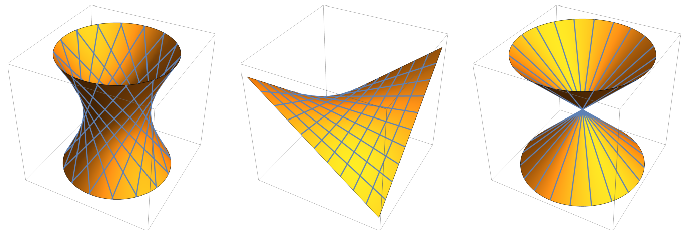
\includegraphics[width=\linewidth]{figures/quadric-surfaces-with-rulings.pdf}

我们在每个曲面上画了一些直线, 以便看出无穷多条直线是怎样分布的. 前两个曲面是光滑的, 第三个则是奇异的, 这一点在曲面上直线的分布中有所反映. 更具体地说, Exercise~\ref{ex:smooth-quadric-iff-doubly-ruled} 论证 $\mathbb{P}^{3}$ 中的二次曲面光滑当且仅当曲面的每一点恰好落在该曲面的两条直线上. 这样的曲面称为\textquotedbl{}双直纹曲面\textquotedbl{}, 前面已经见过一例: Segre 嵌入 $\mathbb{P}^{1}\times\mathbb{P}^{1}\subseteq\mathbb{P}^{3}$, 即上图中的第二个曲面. 实际上, 这本质上是唯一的例子: Exercise~\ref{ex:smooth-quadric-projectively-equivalent-to-segre-surface} 论证 $\mathbb{P}^{3}$ 中每个光滑二次曲面都与 Segre 曲面射影等价. 我们把这两道习题留到下一节, 因为在那里介绍的一些方法会有用.
\end{Example}

\BookPairedNoteLeft{
$K$ 代数闭这一贯穿全书的假设对于 Proposition~\ref{prop:quadric-surfaces-are-covered-by-lines} 至关重要: 将单位球面看成 $\mathbb{R}$ 上的一个二次曲面, 它并不包含任何 (实) 直线.
}{
注意, 若 $d\ge3$, \eqref{eq:degree-two-restriction-to-affine-line-through-point} 的右边还会出现更多系数. 要使 $X$ 包含一条经过 $a\in X$ 的直线, 这些系数也必须为零. 但三个或更多齐次多项式在 $\mathbb{P}^{2}$ 中一般没有公共解.
}
这反映出, 次数 $d\ge3$ 的曲面通常并不是每一点都有曲面中的直线通过. 因此, Proposition~\ref{prop:quadric-surfaces-are-covered-by-lines} 的证明所用的方法在 $d\ge3$ 时失效, 我们需要更精细的技巧.

为了研究 $d\ge3$ 的曲面上的直线, 现在引入一个新工具: 关联簇, 它参数化所有 $d$ 次曲面上的所有直线.

\begin{Definition}{曲面上的直线的关联簇}\leavevmode\label{def:incidence-variety-of-lines-on-surfaces}
对任意 $d\ge1$, $d$ 次曲面上的直线的\emph{关联簇}是 $\mathbb{P}_{3,d}\times\mathrm{G}(2,4)$ 的子集, 定义为
\[
  \Omega_{d}=\{([f],L)\mid L\subseteq\mathcal{V}(f)\}
  \subseteq\mathbb{P}_{3,d}\times\mathrm{G}(2,4).
\]
\end{Definition}

换句话说, $\Omega_{d}$ 的一点 $([f],L)$ 对应一个非零齐次多项式 $f\in K[x_{0},x_{1},x_{2},x_{3}]_{d}$ (相差标量因子视为相同), 以及一条恰好位于消没集 $\mathcal{V}(f)\subseteq\mathbb{P}^{3}$ 上的直线 $L\subseteq\mathbb{P}^{3}$. 为了用代数几何的工具研究关联簇, 首先验证 $\Omega_{d}$ 的确是一个簇.

\begin{Proposition}{曲面上的直线构成一个射影簇}\leavevmode\label{prop:incidence-variety-of-lines-on-surfaces-is-projective}
对 $d\ge1$, $d$ 次曲面上的直线的关联簇 $\Omega_{d}$ 是 $\mathbb{P}_{3,d}\times\mathrm{G}(2,4)$ 的闭子簇. 特别地, $\Omega_{d}$ 是射影簇.
\end{Proposition}
\begin{Proof}
考察 $[f]\in\mathbb{P}_{3,d}$ 和 $L\in\mathrm{G}(2,4)$. 为说明 $\Omega_{d}$ 在 $\mathbb{P}_{3,d}\times\mathrm{G}(2,4)$ 中闭, 我们要用 $\mathbb{P}_{3,d}$ 的坐标 (对应于多项式 $f$ 的系数) 和 $\mathrm{G}(2,4)$ 的 Plücker 坐标 (对应于包含 $\mathrm{G}(2,4)$ 的环境空间 $\mathbb{P}^{5}$ 的坐标) 的多项式约束来刻画 $([f],L)\in\Omega_{d}$ 这一条件.

对某个二维子空间 $V\subseteq K^{4}$ 写 $L=\mathbb{P}(V)$, 并令 $\{v,w\}$ 为 $V$ 的一组基. 我们请读者在 Exercise~\ref{ex:dot-product-map-onto-span} 中证明, 有一个满射 $K^{4}\to V$,
\[
  u\mapsto(u\cdot v)w-(u\cdot w)v,
\]
其中\textquotedbl{}$\cdot$\textquotedbl{}表示 $K^{4}$ 上通常的点积. 若写 $u=(a_{0},a_{1},a_{2},a_{3})$, $v=(b_{0},b_{1},b_{2},b_{3})$, $w=(c_{0},c_{1},c_{2},c_{3})$, 则 $V$ 的任一元素均可写成
\[
  (u\cdot v)w-(u\cdot w)v=(a_{0}p_{00}+\cdots+a_{3}p_{30},\ldots,
  a_{0}p_{03}+\cdots+a_{3}p_{33}),
\]
其中 $p_{ij}=b_{i}c_{j}-b_{j}c_{i}$. 根据 Plücker 映射 $\mathcal{P}_{2,4}$ 的定义, 每个非零的 $p_{ij}$ 都是直线 $L\in\mathrm{G}(2,4)\subseteq\mathbb{P}^{5}$ 的一个 Plücker 坐标 (至多相差一个符号).

条件 $([f],L)\in\Omega_{d}$ 等价于 $f$ 在 $V$ 上消没. 利用 $V$ 中点以 Plücker 坐标 $p_{ij}$ 写出的表达式, 这又等价于对任意 $a_{0},\ldots,a_{3}\in K$ 有
\[
  f(a_{0}p_{00}+\cdots+a_{3}p_{30},\ldots,a_{0}p_{03}+\cdots+a_{3}p_{33})=0.
\]
将它展开为关于 $a_{0},\ldots,a_{3}$ 的多项式: 上述消没成立当且仅当 $a_{0},\ldots,a_{3}$ 的每个单项式的系数都为零. 这些系数是 $L$ 的 Plücker 坐标与 $f$ 的系数的多项式, 因此 $\Omega_{d}$ 在 $\mathbb{P}_{3,d}\times\mathrm{G}(2,4)$ 中闭.
\end{Proof}

我们在最简单的 $d=1$ 情形中把 $\Omega_{d}$ 显式地描述为消没集.

\begin{Example}{$\Omega_{1}$ 的定义方程}\leavevmode\label{ex:equations-defining-incidence-variety-in-degree-one}
任意一点 $[f]\in\mathbb{P}_{3,1}$ 对应线性多项式 $f=\alpha_{0}x_{0}+\cdots+\alpha_{3}x_{3}$, 允许相差标量因子. 此外, 通过 Plücker 映射 $\mathcal{P}_{2,4}$, 任意一点 $L\in\mathrm{G}(2,4)$ 都可以用坐标写为
\[
  L=[p_{01}:p_{02}:p_{03}:p_{12}:p_{13}:p_{23}]\subseteq\mathbb{P}^{5}.
\]
对 $i<j$ 置 $p_{ji}=-p_{ij}$, 并置 $p_{ii}=0$. 依照 Proposition~\ref{prop:incidence-variety-of-lines-on-surfaces-is-projective} 的证明, 可验证 $f$ 在 $L\in\mathrm{G}(2,4)$ 上消没当且仅当
\[
  \alpha_{0}p_{i0}+\alpha_{1}p_{i1}+\alpha_{2}p_{i2}+\alpha_{3}p_{i3}=0
  \qquad\text{对 }i=0,1,2,3.
\]
因此, $\Omega_{1}\subseteq\mathbb{P}_{3,1}\times\mathrm{G}(2,4)$ 是四个多项式的消没集. 这些多项式对来自 $\mathbb{P}_{3,1}=\mathbb{P}^{3}$ 的四个变量 $\alpha_{0},\ldots,\alpha_{3}$ 和来自 $\mathrm{G}(2,4)\subseteq\mathbb{P}^{5}$ 的六个变量 $p_{01},\ldots,p_{23}$ 分别是线性的.
\end{Example}

因为 $\Omega_{d}$ 是乘积 $\mathbb{P}_{3,d}\times\mathrm{G}(2,4)$ 的子簇, 它自然带有到乘积每个因子的投影映射. 接下来, 我们让这两个投影映射相互配合. 第一个投影才是我们真正想研究的: 毕竟, 第一个投影是满射当且仅当对每个 $[f]\in\mathbb{P}_{3,d}$, $\mathcal{V}(f)$ 都包含一条直线. 但下一个结果会表明, 只有理解了第二个投影映射, 才能了解 $\Omega_{d}$ 的结构, 例如它的维数; 而要得到关于第一个投影映射的有用结论, 这些信息不可或缺.

\begin{Proposition}{曲面上的直线的空间的维数}\leavevmode\label{prop:dimension-of-incidence-variety-of-lines-on-surfaces}
对任意 $d\ge1$, 关联簇 $\Omega_{d}$ 不可约, 且
\[
  \dim(\Omega_{d})=\binom{d+3}{3}+2-d=\dim(\mathbb{P}_{3,d})+3-d.
\]
\end{Proposition}
\begin{Proof}
\BookPairedNoteLeft{
这一结果中出现的 $3-d$ 暗示了三次曲面 (即 $d=3$) 之所以特殊的原因.
}{
令 $\pi_{2}:\Omega_{d}\to\mathrm{G}(2,4)$ 为到 $\mathbb{P}_{3,d}\times\mathrm{G}(2,4)$ 的第二个因子的投影的限制. 为证明定理, 我们研究映射 $\pi_{2}$ 的纤维.
}
令 $L\in\mathrm{G}(2,4)$ 为 $\mathbb{P}^{3}$ 中一条直线, 可对某些线性无关的 $\ell_{0},\ell_{1}\in K[x_{0},x_{1},x_{2},x_{3}]_{1}$ 写成 $L=\mathcal{V}(\ell_{0},\ell_{1})$. 注意 $([f],L)\in\pi_{2}^{-1}(L)$ 当且仅当 $f\in\mathcal{I}(L)=\langle\ell_{0},\ell_{1}\rangle$. 换言之, $\pi_{2}^{-1}(L)$ 与 $\mathbb{P}_{3,d}$ 中下面集合的元素所代表的点有自然双射:
\[
  \langle\ell_{0},\ell_{1}\rangle\cap K[x_{0},x_{1},x_{2},x_{3}]_{d}
  \subseteq K[x_{0},x_{1},x_{2},x_{3}]_{d}.
\]
由于 $\langle\ell_{0},\ell_{1}\rangle\cap K[x_{0},x_{1},x_{2},x_{3}]_{d}$ 是 $K[x_{0},x_{1},x_{2},x_{3}]_{d}$ 的线性子空间, $\pi_{2}^{-1}(L)$ 是 $\mathbb{P}_{3,d}$ 的线性子簇, 其维数比 $\langle\ell_{0},\ell_{1}\rangle\cap K[x_{0},x_{1},x_{2},x_{3}]_{d}$ 的向量空间维数少一. 下面计算该维数.

将 $\ell_{0},\ell_{1}$ 扩充为四维向量空间 $K[x_{0},x_{1},x_{2},x_{3}]_{1}$ 的一组基 $\{\ell_{0},\ell_{1},\ell_{2},\ell_{3}\}$. 注意, 存在保持次数的 $K$-代数同构 $K[y_{0},y_{1},y_{2},y_{3}]\to K[x_{0},x_{1},x_{2},x_{3}]$, 它将 $y_{i}$ 映为 $\ell_{i}$. 此同构限制为向量空间同构
\[
  \langle y_{0},y_{1}\rangle\cap K[y_{0},y_{1},y_{2},y_{3}]_{d}
  \cong\langle\ell_{0},\ell_{1}\rangle\cap K[x_{0},x_{1},x_{2},x_{3}]_{d},
\]
所以现在只需计算前者的维数. $\langle y_{0},y_{1}\rangle\cap K[y_{0},y_{1},y_{2},y_{3}]_{d}$ 的一组基由能被 $y_{0}$ 或 $y_{1}$ 整除的单项式给出. 因此, 减去既不能被 $y_{0}$ 整除也不能被 $y_{1}$ 整除的 $d+1$ 个 $d$ 次单项式后, 算得
\[
  \dim\bigl(\langle y_{0},y_{1}\rangle\cap K[y_{0},y_{1},y_{2},y_{3}]_{d}\bigr)
  =\binom{d+3}{3}-d-1.
\]
综上两个段落的论证, 对任意 $L\in\mathrm{G}(2,4)$, 纤维 $\pi_{2}^{-1}(L)$ 是 $\mathbb{P}_{3,d}$ 的一个线性子簇, 其维数为
\begin{equation}\label{eq:dimension-of-lines-projection-fiber}
  \dim(\pi_{2}^{-1}(L))=\binom{d+3}{3}-d-2.
\end{equation}
因此, 由于 $\mathrm{G}(2,4)$ 不可约, 且 $\pi_{2}:\Omega_{d}\to\mathrm{G}(2,4)$ 是满射, 其纤维都不可约且维数相同, Theorem~\ref{thm:projective-domain-irreducible-from-equidimensional-irreducible-fibres} 蕴含 $\Omega_{d}$ 不可约. 知道 $\Omega_{d}$ 不可约之后, 就可以应用 Theorem~\ref{thm:fiber-dimension-equality-on-open-subset}, 它保证存在一个非空开集 $U\subseteq\mathrm{G}(2,4)$, 使
\[
  \dim(\Omega_{d})=\dim(\pi_{2}^{-1}(L))+\dim(\mathrm{G}(2,4))
  \qquad\text{对每个 }L\in U.
\]
因为 $\dim(\mathrm{G}(2,4))=4$, 且 $\pi_{2}$ 的所有纤维都有 \eqref{eq:dimension-of-lines-projection-fiber} 给出的同一维数, 所以
\[
  \dim(\Omega_{d})=\binom{d+3}{3}-d+2.
\]
\end{Proof}

现在可以证明本节的主要结果了.

\begin{Theorem}{每个三次曲面都包含一条直线}\leavevmode\label{thm:cubic-surface-contains-line}
对任意 $f\in K[x_{0},x_{1},x_{2},x_{3}]_{3}$ 中的齐次三次多项式, 至少存在一条直线 $L\subseteq\mathbb{P}^{3}$, 使 $L\subseteq\mathcal{V}(f)$.
\end{Theorem}
\begin{Proof}
令 $\pi_{1}:\Omega_{3}\to\mathbb{P}_{3,3}$ 为到 $\mathbb{P}_{3,3}\times\mathrm{G}(2,4)$ 的第一个因子的投影的限制. 本定理等价于断言 $\pi_{1}$ 是满射. 为导出矛盾, 假设 $\pi_{1}$ 不是满射. 由于 $\Omega_{3}$ 为射影簇, $\pi_{1}(\Omega_{3})$ 在 $\mathbb{P}_{3,3}$ 中闭. 于是由假设可知, $\pi_{1}(\Omega_{3})$ 是不可约簇 $\mathbb{P}_{3,3}$ 的真闭子簇. 因此 (Exercise~\ref{ex:quasiprojective-dimension-monotone-and-strict-for-proper-closed-subvariety}), 有
\[
  \dim(\pi_{1}(\Omega_{3}))<\dim(\mathbb{P}_{3,3})=19.
\]
但是, 由于 $\dim(\Omega_{3})=19$ (Proposition~\ref{prop:dimension-of-incidence-variety-of-lines-on-surfaces}), 而 $\dim(\pi_{1}(\Omega_{3}))<19$, Theorem~\ref{thm:fiber-dimension-lower-bound} 蕴含 $\pi_{1}$ 的每个非空纤维的维数至少为一. 另一方面, Exercise~\ref{ex:cubic-surface-containing-exactly-three-lines} 给出一个三次多项式 $f\in K[x_{0},x_{1},x_{2},x_{3}]_{3}$ 的明确例子, 使 $\mathcal{V}(f)$ 包含有限且非零条直线. 这说明纤维 $\pi_{1}^{-1}([f])$ 的维数为零, 矛盾. 因此 $\pi_{1}$ 为满射, 如所断言.
\end{Proof}

本节至此证明了, 当 $d\le3$ 时, 对任意 $[f]\in\mathbb{P}_{3,d}$ 都存在一条直线 $L\subseteq\mathcal{V}(f)$. 最后陈述 $d>3$ 时的情形, 把证明留给读者作为练习.

\begin{Proposition}{多数高次曲面不包含直线}\leavevmode\label{prop:high-degree-surfaces-containing-lines-have-large-codimension}
对 $d>3$, 使 $\mathcal{V}(f)\subseteq\mathbb{P}^{3}$ 包含直线的点 $[f]\in\mathbb{P}_{3,d}$ 的集合是 $\mathbb{P}_{3,d}$ 的闭子簇, 其余维至少为 $d-3$.
\end{Proposition}
\begin{Proof}
Exercise~\ref{ex:codimension-of-high-degree-surfaces-containing-lines}.
\end{Proof}

\BookPairedNote{
换句话说, 对 $d>3$, $\mathbb{P}_{3,d}$ 中存在由点 $[f]$ 构成的一个非空开子集, 使对应的曲面 $\mathcal{V}(f)\subseteq\mathbb{P}^{3}$ 一条直线也不包含.
}{
直观上, 曲面越弯曲, 就越不容易包含一条直线.
}
还可以换一种说法: 若 $f\in K[x_{0},x_{1},x_{2},x_{3}]$ 是次数为 $d>3$ 的齐次多项式, 则要使 $\mathcal{V}(f)\subseteq\mathbb{P}^{3}$ 包含一条直线, 它的系数必须满足某些非平凡的多项式关系. 而且随着 $d$ 增大, 相对于 $\mathbb{P}_{3,d}$ 的维数, 使 $\mathcal{V}(f)$ 包含直线的 $[f]\in\mathbb{P}_{3,d}$ 的集合越来越小, 也就是说, 为保证 $\mathcal{V}(f)$ 包含一条直线, $f$ 的系数必须满足越来越多的关系.

\BookExerciseHeading
\begin{BookExercises}
  \item\label{ex:two-lines-through-point-on-complex-quadric} 考察二次曲面 $X=\mathcal{V}(x_{0}^{2}-x_{1}^{2}-x_{2}^{2}-x_{3}^{2})\subseteq\mathbb{P}_{\mathbb{C}}^{3}$, 它的实点是 $\mathbb{A}_{0}^{3}$ 内的单位球面. 在 $X$ 中构造经过 $a=[1:0:0:1]$ 的两条不同的直线.
  \item\label{ex:lines-on-quadric-cone-pass-through-vertex} 考察二次曲面 $X=\mathcal{V}(x_{1}^{2}+x_{2}^{2}-x_{3}^{2})\subseteq\mathbb{P}_{\mathbb{C}}^{3}$, 它的实点限制在仿射开片 $\mathbb{A}_{0}^{3}$ 上是顶点位于原点的圆锥面. 证明 $X$ 中的每条直线都经过 $[1:0:0:0]$, 并用这一事实解释为什么 $X$ 中除 $[1:0:0:0]$ 以外的每一点都包含在 $X$ 的唯一一条直线中.
  \item\label{ex:dot-product-map-onto-span} 令 $v,w\in K^{4}$. 证明把 $u$ 送到 $(u\cdot v)w-(u\cdot w)v$ 的映射 $K^{4}\to K^{4}$ 是到 $v$ 和 $w$ 的张成空间上的满射.
  \item\label{ex:equations-defining-incidence-variety-in-degree-two} 写出 $\Omega_{2}$ 作为 $\mathbb{P}_{3,2}\times\mathrm{G}(2,4)$ 的子簇的定义方程.
  \item\label{ex:fibers-of-different-dimensions-for-quadric-lines} 举出 $[f]\in\mathbb{P}_{3,2}$ 的一个例子, 使纤维 $\pi_{1}^{-1}([f])\subseteq\Omega_{2}$ 的维数为一, 并举一个例子使该纤维的维数为二.
  \item\label{ex:cubic-surface-containing-exactly-three-lines} 考察三次曲面 $X=\mathcal{V}(x_{0}^{3}-x_{1}x_{2}x_{3})\subseteq\mathbb{P}^{3}$.
  \begin{enumerate}
    \item 证明 $X\cap\mathcal{V}(x_{0})$ 是 $\mathbb{P}^{3}$ 中三条直线的并.
    \item 证明仿射限制
    \[
      X_{0}=\mathcal{V}(1-x_{1}x_{2}x_{3})\subseteq\mathbb{A}^{3}
    \]
    不包含任何 (仿射) 直线. (提示: 任意仿射直线都可参数化为 $\{a+tb\mid t\in K\}$, 其中 $a,b\in\mathbb{A}^{3}$ 且 $b\ne0$.)
    \item 由此得出 $X$ 恰好包含三条直线.
  \end{enumerate}
  \item\label{ex:codimension-of-high-degree-surfaces-containing-lines} 证明 Proposition~\ref{prop:high-degree-surfaces-containing-lines-have-large-codimension}. (提示: 所讨论的集合是 $\pi_{1}(\Omega_{d})\subseteq\mathbb{P}_{3,d}$.)
\end{BookExercises}
